\section{Durchführung}
\label{sec:Durchfuehrung}
\subsection{Resonanzfrequenz}
\label{sec:Resonanzfrequenz}
\begin{figure}[h]
	\centering
		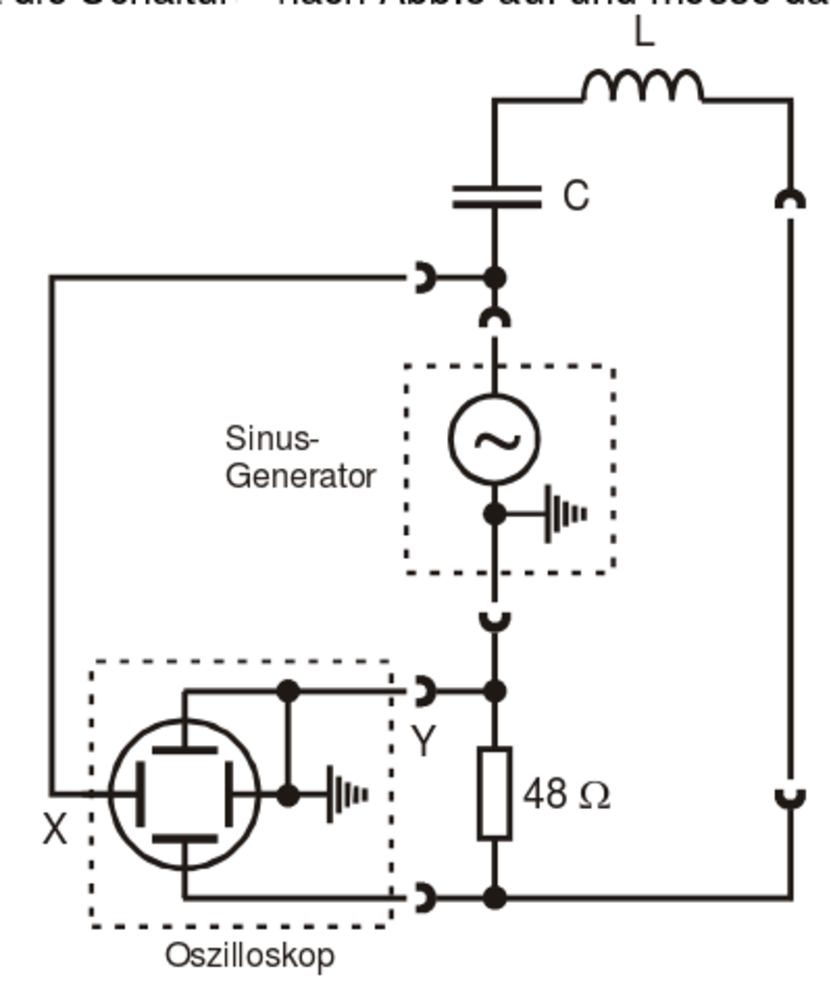
\includegraphics[width=0.5\textwidth]{Bilder/Resonanzfrequenz.pdf}
		\caption{Schaltung zur Bestimmung der Resonanzfrequenz. \cite{v355}} 
\label{fig:resonanzfrequenz}
\end{figure}
Vor Messbeginn muss die feste Resonanzfrequenz eines Schwingkreises gemessen und anschließend die des anderen Schwingkreises darauf abgestimmt werden. 
Dazu wird die in Abbildung \ref{fig:resonanzfrequenz} gezeigte Schaltung aufgebaut. \\
Zur Abschätzung wird der festlegende Schwingkreis durch den Frequenzgenerator zum Schwingen angeregt. 
Durch Variieren der Frequenz am Generator ändert sich die am Widerstand $R_1$ abfallende Spannung $U_\mathup{R_1}(t)$. 
Die am Generator eingestellt Frequenz entspricht der Resonanzfrequenz $f_\mathup{Res}$ des Systems, wenn die Spannung $U_\mathup{R_1}(t)$ maximal wird.

Die Feineinstellung wird mit dem X-Eingang des Oszilloskopes vorgenommen.
Dazu wird das Oszilloskop in XY-Betrieb umgeschaltet. 
Beiden Eingängen wird nun eine Spannung geliefert; 
die Widerstandsspannung $U_\mathup{R_1}(t)$ und die Erregerspannung $U(t)$ überlagern sich und werden gegeneinander aufgetragen. 
Auf dem Oszilloskop wird diese Überlagerung als \textsc{Lissajous}-Figur sichtbar, nach derem Aussehen sich die Phasendifferenz zwischen Generator- und Schwingkreisstrom beurteilen lässt. 
Der Resonanzfall tritt ein, wenn für die Phasendifferenz $\Delta{\phi}=0$  gilt und eine Gerade auf dem Bildschirm erscheint. 
Diese verläuft im ersten und dritten Quadranten des Bildschirms.
Um den zweiten Schwingkreis auf dieselbe Frequenz einzustellen, wird die Schaltung mit diesem Schwingkreis erneut aufgebaut. 
Über eine variable Kapazität wird nach gleichem Verfahren die vorher bestimmte Resonanzfrequenz eingestellt.

\subsection{Verhalten der Schwingungsenergie}
\begin{figure}[h]
	\centering
		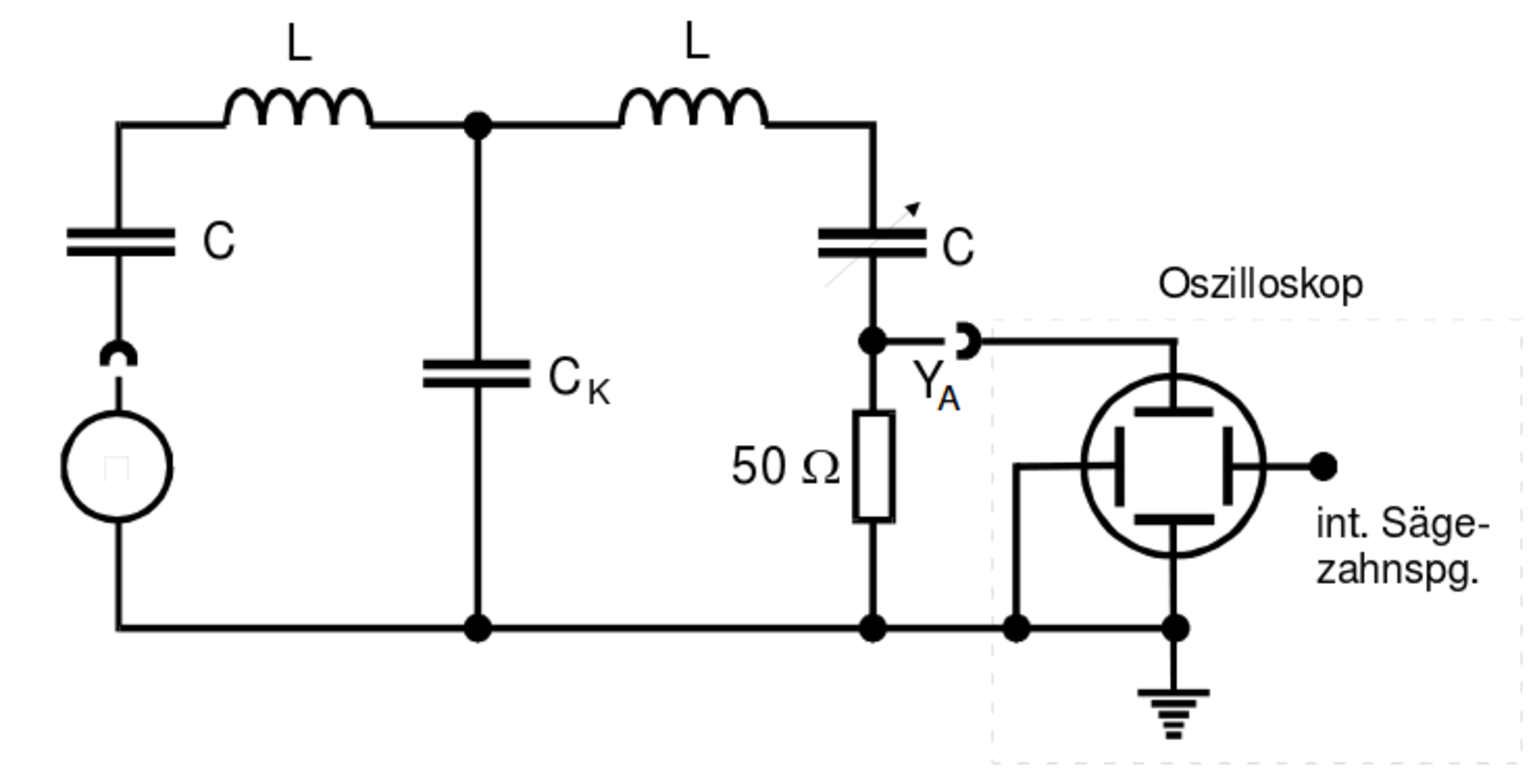
\includegraphics[width=0.8\textwidth]{Bilder/Versuchsaufbau.pdf}		
\caption{Schaltung zur Untersuchung gekoppelter Schwingkreise. \cite{v355}}
	\label{fig:versuchsaufbau}
\end{figure}
Für den ersten Versuchteil wird die Schaltung wie in Abbildung \ref{fig:versuchsaufbau} benötigt. 
Mit einem Rechteckimpuls wird ein Kreis zum Schwingen angeregt. 
Am ohmschen Widerstand fällt eine Spannung $U_\mathup{R_2}(t)$ ab, die durch das Oszilloskop dargestellt wird. 
Anschließend werden die Schwingungsmaxima pro Schwebungsperiode bei variablen Kopplungskapazitäten $C_\mathup{K}$ abgezählt.

Die Beschreibung dieser Schwebung zeigt das Verhalten der im Schwingkreis gespeicherte Energie.

\subsection{Frequenzen der Fundamentalschwingungen in Abhängigkeit der Koppelkapazität $C_\text{K}$}
Der zweite Versuchsteil basiert auf derselben Schaltung, die Schwingung wird nun jedoch mit einem Sinusgenerator angeregt.
Die Kapazität $C_\mathup{K}$ wird erneut variiert. 
Für jede Kapazität wird die \textsc{Lissajous}-Figur betrachtet und die Frequenz des Generators so eingestellt, dass der Phasenunterschied $\phi=0$ bzw. $\phi=\pi$ beträgt. 
Bei $\phi=0$ ergibt sich dieselbe Figur wie in Abschnitt \ref{sec:Resonanzfrequenz} erläutert; 
für $\phi=\pi$  ergibt sich ebenfalls eine Gerade, die jedoch im zweiten und vierten Quadranten verläuft, also an der $U_\mathup{R_2}(t)$ gespiegelt ist.

\subsection{Frequenzabhängigkeit der Ströme}
\label{sec:Frequenzgenerator}
Der dritte Versuchteil basiert, wie Teil 1 und 2, auf der Schaltung in Abbildung \ref{fig:versuchsaufbau}. Die Einstellungen des Generators werden so geändert, dass dieser in $\SI{20}{\milli\second}$ ein Frequenzband von $10-80\,\si{\kilo\hertz}$ durchläuft.
Dabei wird die am Widerstand abfallende Spannung $U_\mathup{R_2}(t)$ gegen die Zeit $t$ -- ein Maß für die Frequenz $f$ -- aufgetragen, sodass ein Spannungs-Frequenz-Diagramm entsteht, welches in Kapitel \ref{sec:erzwungen} beschrieben wird.
Anschließend wird die Kopplungskapazität $C_\text{K}$ variiert und die Zeitkoordinaten $t_+$ und $t_-$ der auftretenden Maxima notiert, sodass mit sämtlichen Kopplungskapazitäten $C_\text{K}$ gemessen wird.
